\section{PCIe and InfiniBand}
\label{sec:pcie}

This section discusses relevant details of PCI Express and InfiniBand, and
discusses what PCIe events are measured by Intel's PCIe counters on different
CPU generations.

\subsection{PCI Express}
PCIe is a serial point-to-point interconnect which is commonly used to connect
peripheral devices to a CPU. The bandwidth of a PCIe link is determined by two
factors: the link width and the PCIe generation. The link width speficies the
number of parallel lanes in the interconnect---the bandwidth of the link is
simply the per-lane bandwidth multiplied by the number of lanes. The PCIe
generation can be any number between 1 and 3, with PCIe 3.0 being the newest
generation at the time of writing. The transfer rate of a PCIe lane has
increased with each PCIe generation; Table~\ref{table:pcie} shows the transfer
rate of different PCIe generations and the bandwidth of a single lane of this
generation. As diffenent PCIe generations use different physical layer encodings
(8b/10b for PCIe 1.0 and 2.0, 128b/130b for PCIe 3.0), the relation between the
transfer rate and useful bandwidth of a PCIe lane depends on the generation. 

\begin{table}
\begin{center}
    \begin{tabular}{p{2.5cm} p{1.5cm} p{2.5cm}}
	\textbf{Generation} & \textbf{Bitrate} & \textbf{Lane bandwidth}\\
    \hline
	PCIe 1.0 & 2.5 GT/s & 250 MB/s \\
	PCIe 2.0 & 5 GT/s & 500 MB/s \\
	PCIe 3.0 & 8 GT/s & 984.6 MB/s \\
    \end{tabular}
\caption{Transfer rate and per-lane bandwidth of different PCIe generations}
\label{table:pcie}
\end{center}
\end{table}

\subsubsection{PCIe protocol}
PCIe is a layered protocol and consists of a physical layer, a link layer,
and a transport layer. The link layer uses credit-based flow control and
acknowledgments to provide reliable delivery to the transport layer.
Figure~\ref{fig:pcie-tlp} shows the structure of a PCIe 3.0 transaction layer
packet (PCIe TLP). In addition to the data payload, the packet includes physical
layer framing, a link layer sequence number (for reliability), a transport layer
header, and checksum at both the transport and link layer.

For the purposes of this paper, we assume that there are two types of PCIe
operations: memory read and memory write. The type of operation and the memory
address (in the peer's virtual memory) to read or write from is specified
in the transaction layer header. Therefore, the transaction layer
header can be either 12 or 16 bytes depending on whether 32-bit or 64-bit
addressing is used.  As almost all modern servers use 64-bit addressing, we
assume that the size of the transaction layer header is 16 bytes.

Note that the exact method of generating PCIe read and write transactions is
different for CPUs and NICs. The two common methods for generating these
transactions are Mapped Memory I/O (MMIO) and Direct Memory Access (DMA). MMIO
is used by the CPU to read or write the NIC's memory, whereas the NIC uses
DMA to read or write the CPU's memory. The efficiency of these two methods in
terms of CPU utilization (CPU utilization is reduced if a CPU-initiated MMIO
write can be replaced by a NIC-initiated DMA read) and PCIe bandwidth (MMIO
operations are restricted to a cacheline granularity) is different, which leads
to interesting optimizations and tradeoffs~\ref{sec:measurements}.

From Figure~\ref{fig:pcie-tlp}, it is clear that the minimum TLP overhead of
a PCIe packet is 30 bytes. This overhead is comparable to the common size of
data items used in networked services such as memcached~\cite{Nishtala:nsdi2013}
and RPCs~\cite{Flajslik:usenix2013}. Understanding and mitigating this overhead
can help in to designing RDMA-based communication protocols and networked
systems, as we will show in Section~\ref{sec:measurements}.

\begin{figure}
	\centering
	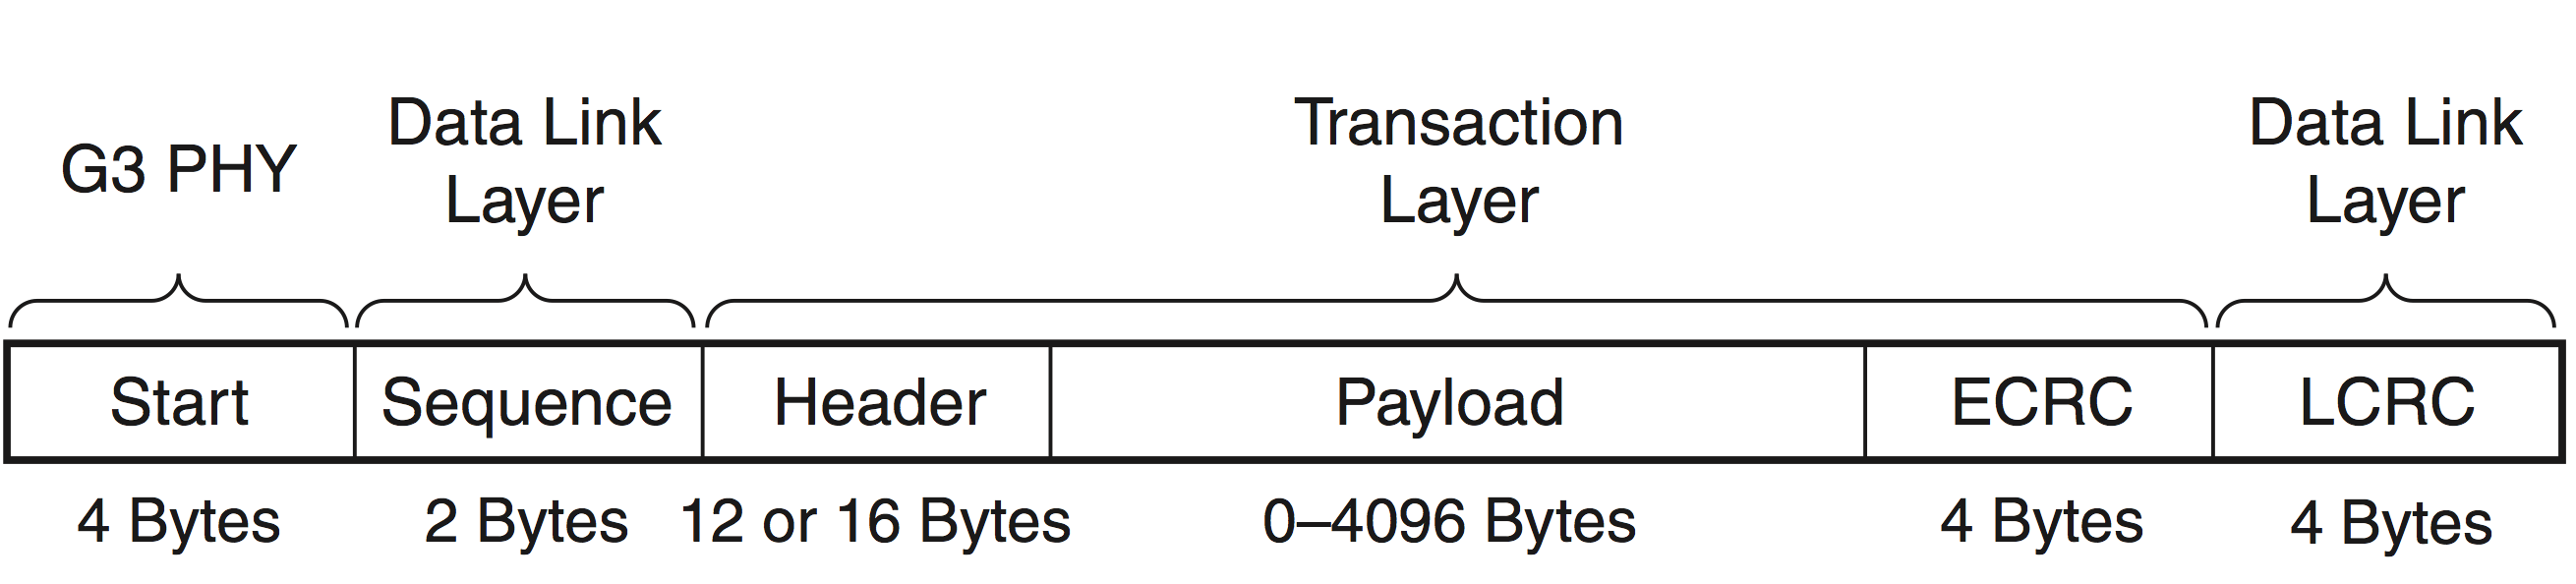
\includegraphics[width=.48\textwidth]{figures/pcie-tlp.png}
	\caption{\textbf{Structure of a PCIe TLP. The diagram was copied from~\cite{www-xilinx-pcie}}}
	\label{fig:pcie-tlp}
\end{figure}

\subsection{InfiniBand}
InfiniBand is standard for high-speed communication, commonly deployed between
two servers in a datacenters. InfiniBand focuses on low-latency and
high-bandwidth communication. The InfiniBand adapters used in this work have 56
Gbps of peak theoretical bandwidth per port, with $\sim$ 2 microseconds of
round-trip latency. All InfiniBand-compliant adapters must also provide RDMA.

\subsubsection{InfiniBand protocol and verbs}
Similar to PCIe, InfiniBand is a layered protocol. The header format of an
InfiniBand packet depends on several factors including the transport (connected
or datagram) and the type of RDMA operation (RDMA write or read or atomic). We
omit repeating all the header fields in this paper because they are irrelevant
from the PCIe point of view.

InfiniBand operations are also called ``verbs''. There are two main types of
verbs---memory verbs (RDMA READ and WRITE), which specify the remote memory
address to operate on, and messaging verbs (SENDs and RECVs), which behave
somewhat similarly to traditional UNIX sockets. The remote address to which the
payload of a SEND is written to is specified in a RECV that was previously
posted by the remote host.

\subsubsection{CPU-NIC interaction for RDMA}
InfiniBand communication uses queue pairs at the end hosts. To initiate an
InfiniBand operation, a user-level NIC driver at the requester host creates
a Work Queue Element (WQE) in host memory\footnote{We call the memory (cache
or DRAM) connected to a host CPU ``host memory'' and the memory (SRAM) of a NIC
``device memory''.}. The size of the WQE depends on several factors:
the type of InfiniBand operation, the InfiniBand transport, and whether or not
the data payload is ``inlined'' in the WQE. For example, excluding the optional
inlined data payload, an RDMA write WQE is 36 bytes in size. It consists of
16 byte control segment which contains the operation opcode and the queue pair
number of the remote peer's queue pair, a 16 byte ``remote address'' segment
which contains the address and permissions for the remote memory area to write
the data payload to, and a 4 byte data length field.


The WQE needs to be transferred from host memory to device memory over the
PCIe interconnect. There are 3 possible methods of doing this.

\begin{enumerate}
\item \textbf{Doorbell method}: The CPU writes to a memory-mapped register in
the NIC, alerting it of the availability of a new WQE. The NIC reads the WQE via
a PCIe DMA read. This requires 2 PCIe transactions: a PCIe write from CPU to NIC,
and a PCIe read from NIC to CPU.
\item \textbf{BlueFlame method}: Using Mellanox's terminology, in the BlueFlame
method, the CPU writes the entire WQE to the NIC via MMIO. This only requires
1 PCIe write and removes $\sim$200-400ns of PCIe read latency from the critical
path.
\end{enumerate}

After processing the WQE, the NIC writes a completion queue element to the
host's memory. This is done using a PCIe DMA write.

\subsection{PCIe counters}
Intel's Xeon CPUs provide counters for several useful PCIe events. The PCIe
counters measure activity between the CPU's PCIe controller and the L3 cache.
As all communication with the L3 cache needs to be done at a cacheline
granularity, the counters can miss some critical information. For example,
irrespective of whether the NIC reads a 4-byte or 64-byte chunk of host memory,
the counters report 1 PCIe read. Further, the older CPU generations have fewer
working counters.

The PCIe counters are easily accessible using the \texttt{pcm-pcie.x} utility
which is a part of Intel's freely available Performance Counter
Monitor~\cite{www-intel-pcm}. As the behavior of these counters is not well
understood or documented, we include a description of 3 useful counters here.

\begin{itemize}
\item \textbf{PCIeRdCur}: The number of partial cacheline DMA reads done by
the device. This counter works in the same way on both Haswell and
SandyBridge/IvyBridge CPUs.
\item \textbf{PCIeItoM}: The number of full cacheline DMA writes done by the
the device. On SandyBridge/IvyBridge, there is no way to count the number of
partial cacheline DMA writes.
\item \textbf{WiL}: The number of partial and full cacheline MMIO transfers
done by the CPU. This counter is disabled on SandyBridge/IvyBridge.
\end{itemize}
